\chapter{Introduction}
In bioinformatics, especially in bioinformatics for proteomics, databases are becoming increasingly important. One research topic of Medical Bioinformatics of the Ruhr-University Bochum, located at Medizinisches Proteom-Center, is the investigation of relationships between biomarkers and diseases. In other words, which biomarkers are related to a specific disease. To answer this question the database \ac{BIONDA} was developed. Using this application, it is possible to search for disease-biomarker-relations in scientific publications. The target group of \ac{BIONDA} are not only scientists worldwide but also the pharmaceutical industry and affected persons worldwide \citep{Bionda}. Unfortunately, the problem is that the current source database for disease entities, namely \ac{UniProt}, does not contain enough disease terms. Furthermore, another problem is that there are too few synonyms of a disease. Beside diseases as an entity, the database also contains genes, \ac{miRNA} and proteins as biomarker entities. Therefore, this work deals with the integration of an independent alternative disease database into the existing structure of \ac{BIONDA}. In a first step, suitable disease databases needs to be identified, then compared under defined criteria and a suitable database needs to be selected. In a second step, the new source database will be integrated into BIONDA, which includes, among other things, adapting the tables of the database. These two steps are explained in more detail in chapter \ref{chapter_methods}. At first, basics are presented, which are necessary for further understanding of this work. First of all, the term \textit{disease} will be explained. Since there is no unique definition, this term is described by disease subcategories. As mentioned, the goal of the research is the investigation of relationships between diseases and so-called \textit{biomarkers}. Thus, section 1.2 defines the term biomarker. Finally, an overview of the application BIONDA will be drawn. The following chapter will discuss the available disease databases and the process of defining criteria, which will make sure a suitable replacement for the current disease database. In chapter \ref{chapter_methods} all technical aspects will be explained in detail and the necessary steps to build the new database will be discussed. Finally, the results will be presented and a discussion to this work will be given.

\section{Diseases}
When searching the term \textit{disease}, it quickly becomes clear that this is not easy to define. The term is used synonymously with other terms, which makes it difficult to formalize a definition. If one visits the website of Human Disease Ontology \citep{noauthor_disease_nodate} it becomes clear that a disease can be categorized into multiple subcategories. Thus, this section describes the subcategories of the highest level of disease classification. Syndromes or physical disorders are defined as diseases, too. Instead of a general definition, parts of the subcategories of the superordinate category disease are presented. Figure \ref{fig:disease_tree} provides an overview of the subcategories. Disease by infectious agents is a group of diseases \enquote{that is caused by the invasion of a host by agents whose activities harm the hosts tissues (that is, they cause \textit{disease}) and can be transmitted to other individuals (that is, they are \textit{infectious})} \citep{health_us_understanding_2007}. The agents can be categorized into five types, such as: viruses, bacteria, fungi, protozoa and helminths \citep{charles_a_janeway_infectious_2001}. The most known diseases of this subcategory include \ac{HIV} and \ac{AIDS}. \\

Continuing with the next category, disease of anatomical entity, Parkinson is one of the most researched disease in this category. Parkinson is described as \enquote{a chronic progressive neurological disease chiefly of later life that is linked to decreased dopamine production in substantia nigra and is marked especially by tremor of resting muscles, rigidity, slowness of movement, impaired balance} \citep{noauthor_definition_nodate}. Thus this category of diseases refers to ones that develop over time.\\

\begin{figure}[H]
\centering
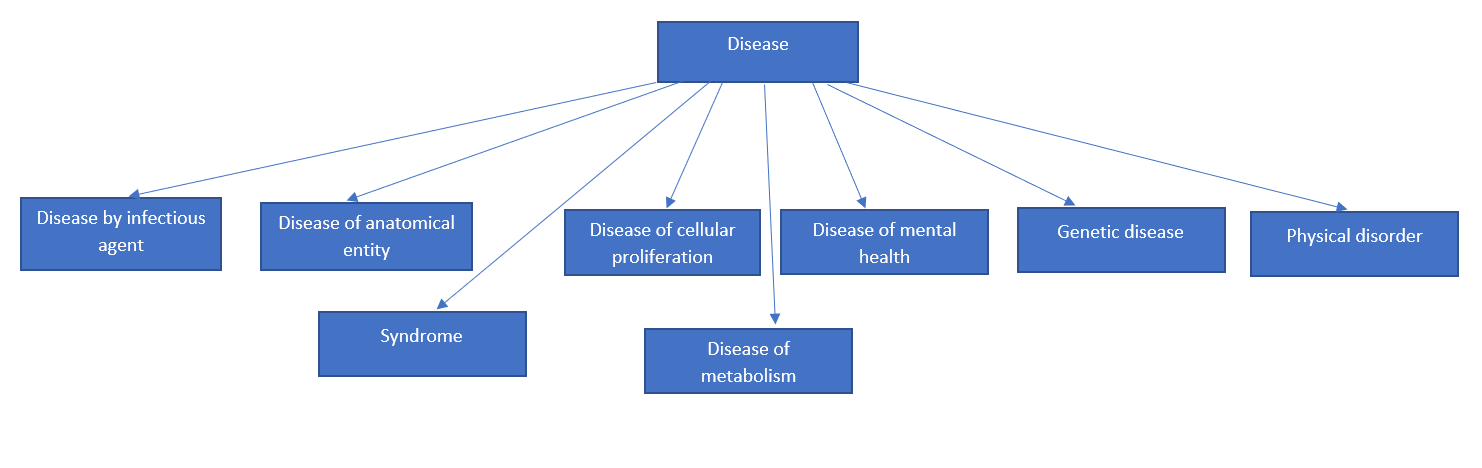
\includegraphics[scale=0.6]{bilder/Disease.PNG}
\caption{General classification of diseases according to the Disease Ontology}
Source: \citep{noauthor_disease_nodate}
\label{fig:disease_tree}
\end{figure}

Cancer is one of the most known diseases, which falls into the category disease of cellular proliferation. Especially it is a disease \enquote{in which abnormal cells divide without control and can invade nearby tissue. Cancer cells can also spread to other parts of the body} \citep{noauthor_nci_2011}. Hereinafter, the subcategory describes diseases in which cells proliferate abnormally. On one hand, mental illnesses \enquote{are conditions that affect your thinking, feeling, mood, and behavior} \citep{noauthor_mental_nodate}, which include diseases such as dementia or depression and on the other hand, down syndrome is an example of a genetic disease. A genetic disease \enquote{is a disease caused in whole or in part by a change in the \ac{DNA} sequence away from the normal sequence} and \enquote{can be caused by a mutation in one gene mutations, in multiple gene combination of gene mutations or damage to chromosomes} \citep{noauthor_genetic_nodate}. \\

The cleft palate-lateral synechia syndrome is a physical disorder and \enquote{is a congential malformation syndrome characterized by the association of cleft palate and intra-oral lateral synechiae connecting the free borders of the palate and the floor of the mouth} \citep{reserved_orphanet_nodate}.\\

Understanding the multiple categories of a disease one can now break it further down to elements, which may be already in the human system or emerge due a disease. This quantity will be discussed in detail in the next section.

\section{Biomarkers}
Biomarkers are processes, structures or any substances that can be measured in any living body. Especially, elements which influence or predict the result of a disease are called biomarkers, too. \citep{noauthor_biomarkers_nodate}. Biomarkers are used, among other purposes, to provide information on the health status of a patient or to determine the progress of a disease  \citep{atkinson_biomarkers_2001, mayeux_biomarkers:_2004}. Biomarkers can be used, for instance,  to determine the stage of a disease. This is done, for example, by measuring specific antigen in the blood concentration. To determine the progress of a disease, for example prostate cancer, a specific antigen (antigen-125) \citep{atkinson_biomarkers_2001} is examined to determine the growth of a tumor. 

\begin{figure}[H]
\centering
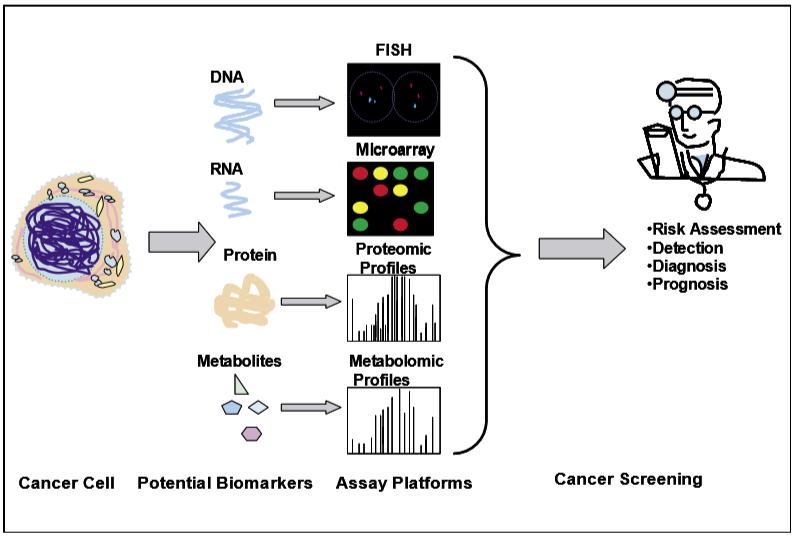
\includegraphics[scale=0.7]{bilder/Biomarker.PNG}
\caption{Relationship between diseases and biomarkers}
Source: \citep{maruvada_biomarkers_2005}
\label{fig:disease_biomarker}
\end{figure}

Figure \ref{fig:disease_biomarker} further illustrates the relationship between biomarkers and diseases. There are different types of biomarkers. Prognostic biomarkers are used to calculate the probability of a reoccurring disease. They are used also to measure the progress of a specific medical condition, which can be of specific value to the scientists. An example of such a biomarker is the Gleason-Score \citep{group_prognostic_2016}. \\

Predictive biomarkers are to identify which and how individuals could react to an exposure of a medical product or a specific agent \citep{group_predictive_2016}. The mutations of cystic fibrosis transmembrane conductance regulator are an example of such a biomarker \citep{group_predictive_2016}. This can also be said to pharmacodynamic biomarkers which are used to show that an individual has positive or negative reaction to a medical product or an environmental agent. Hemoglobin A1c is an example of such a biomarker  \citep{group_pharmacodynamicresponse_2016}. The last type, namely surrogate endpoints, is \enquote{an indicator or sign used in place of another to tell if a treatment works.} \citep{noauthor_nci_2011}. Blood pressure is an example of a surrogate endpoint \citep{noauthor_surrogate_nodate}. Since BIONDA deals with the relationship between biomarkers and diseases it is crucial to understand, which role biomarkers have. \\

In this case one can note that biomarkers can be crucial for the diagnosis of a disease. Analyzing for example the blood or urine of a patient the resulting biomarkers are used as biological factors, which for example represent the stage of disorder. These biomarkers can also be used to warn patients of possible diseases in advance \citep{mayeux_biomarkers:_2004}.


\section{BIONDA}
The database BIONDA, which is accessible via a web application, was developed by the Medical Bioinformatics Department of the Ruhr-University Bochum. The motivation of it was to investigate the relationships between diseases and biomarkers. The target group are scientists worldwide, who can use this database for their research. Further target groups should not only be the pharmaceutical industry but also affected persons. Figure 3 shows the general architecture of BIONDA.

\begin{figure}[H]
\centering
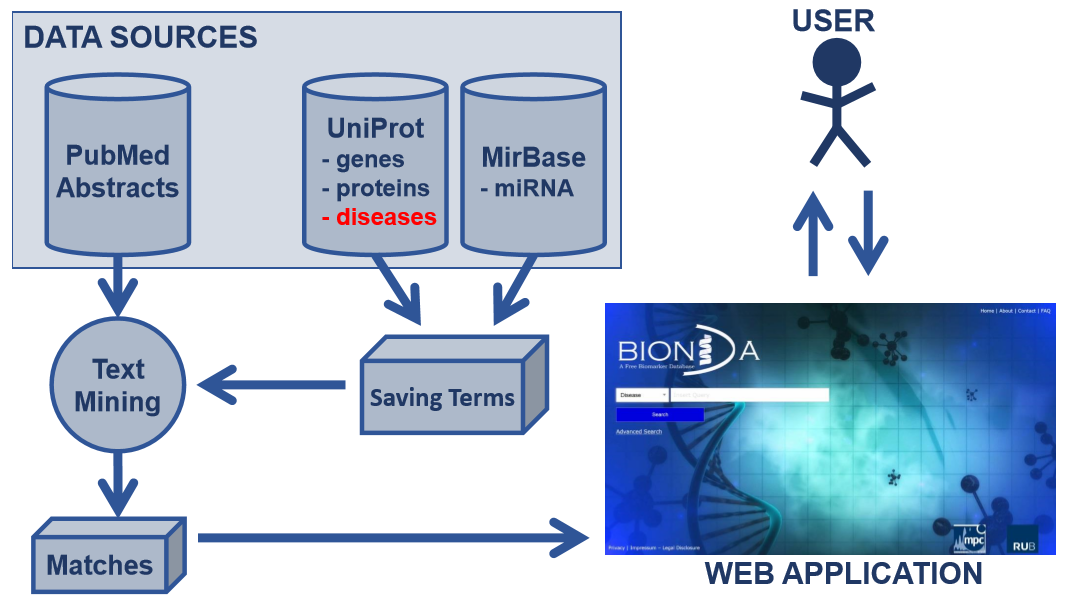
\includegraphics[scale=0.6]{bilder/BIONDA.png}
\caption{Overview of BIONDA}
Source: \citep{Bionda}
\label{fig:Overview_Bionda_Infra}
\end{figure}

\ac{BIONDA} allows to search for relations between specific diseases and biomarkers in scientific publications. This is done by submitting a disease or biomarker name as a search term in the BIONDA web application. This is achieved by parsing abstracts of publications and perform text mining to match papers with specific search terms. The search can also be restricted to a sentence-wise or abstract-wise biomarker match. Depending on the search category, the search returns the disease metadata, but the relationship between the metadata is interpreted differently. The search is by default using the abstract-wise option, which makes sure that the desired biomarker and the associated disease were mentioned in the abstracts of the publications. When searching with abstract-wise, the evidence is not directly displayed, because the abstracts are indexed via the \ac{PMID}. However, using the sentence-wise option \ac{BIONDA} makes sure that the term is mentioned in the same sentence of the abstract. This allows the user a more refined search.  However, both option make it possible to draw relations between biomarkers and diseases.  One of the most important metadata in \ac{BIONDA} is the co-occurence-based p-value \citep{pvalue}. This resembles a score to the user, which is calculated using the $\chi^2$ test \citep{chisquaredtest} and is based on the co-occurence of markers and diseases. This test requires the true positive, true negative, false positive, and false negative of a specific biomarker and disease pair \citep{bionda_web}.

\begin{itemize}
\item{True positives are defined as the number of a matched pair of biomarker X and a disease Y in the same abstract or sentence of an abstract, }
\item{False negatives are defined as the number of search hits from a biomarker X but without disease Y, in the same abstract or sentence of an abstract, }
\item{False positives are defined as the number of hits from a disease Y but without the biomarker X, in the same abstract or sentence of an abstract, }
\item{True negatives are defined as the number of search hits from all other pairs \citep{bionda_web}.}
\end{itemize}

In general the more matches are achieved of a biomarker and disease pair, the better the p-value and thus the score.\\

The current database which is used by \ac{BIONDA} is \ac{UniProt}. \ac{UniProt} is a data resource for protein sequences, whose data is freely accessible. It gets updated monthly and is provided by the \ac{EMBL-EBI}, the \ac{SIB} and the \ac{PIR}. Over 100 people work on different aspects of this specific database. Originally, each institute managed its own database. Yet, in 2002 they decided to pool them together, which made \ac{UniProt} become a collection of them all \citep{noauthor_uniprot_nodate}. The main aspect which is of importance for this project are the 5,466 disease entries in the \ac{UniProt} database. This total number of disease entries need to be increased by the new database. 

\section{Aim of this Project}
In the first part of this project, the goal is to determine a suitable database for \ac{BIONDA}, which contains a large number of diseases. This new disease database should make it possible to search for a larger amount of diseases within \ac{BIONDA}. \ac{BIONDA} already uses a database but the total number of disease entries needs to be increased. Thus, the main target of this project is to find a larger disease database than \ac{UniProt}, which is the currently used disease resource \citep{Bionda}. In order to find a suitable database, a rough overview of existing databases will be made first, in that way it is possible to choose a suitable option. After that the integration process needs to be explained in detail. The following chapters will discuss which database are available and the requirements of these.